\documentclass[
a4paper,
12pt
]{scrartcl}


\usepackage{tikz}
\usetikzlibrary{arrows,automata}
\usepackage[latin1]{inputenc}
\usepackage[T1]{fontenc}
\usepackage{ae,aecompl}
\usepackage{amsmath,amssymb,amstext}
\usepackage{algorithm}
\usepackage{algpseudocode}
\usepackage{float}
\usepackage{psfrag}
\usepackage{listings}
\usepackage{color}
\usepackage[automark]{scrpage2}
\usepackage{smartdiagram}
\usepackage{ifpdf}
\usepackage{xcolor,colortbl}

\makeatletter
\def\BState{\State\hskip-\ALG@thistlm}
\makeatother

\definecolor{codegreen}{rgb}{0,0.6,0}
\definecolor{codegray}{rgb}{0.5,0.5,0.5}
\definecolor{codepurple}{rgb}{0.58,0,0.82}
\definecolor{backcolour}{rgb}{0.95,0.95,0.92}

\definecolor{grayself}{rgb}{0.9,0.9,0.9}
\newcommand{\gray}{\cellcolor{grayself}}  %{0.9}

\lstdefinestyle{prism}{
    backgroundcolor=\color{backcolour},
    commentstyle=\color{codegreen},
    keywordstyle=\color{magenta},
    numberstyle=\tiny\color{codegray},
    stringstyle=\color{codepurple},
    basicstyle=\footnotesize,
    breakatwhitespace=false,
    breaklines=true,
    captionpos=b,
    keepspaces=true,
    numbers=left,
    numbersep=5pt,
    showspaces=false,
    showstringspaces=false,
    showtabs=false,
    tabsize=2
}

\lstdefinelanguage{Prism}
{
  % list of keywords
  morekeywords={
  bool,C,ceil,const,ctmc,double,dtmc,endinit,endmodule,endrewards, endsystem,F,false,floor,formula,G,global,I,init,int,label,max,mdp,min, module,nondeterministic,P,Pmin,Pmax,prob,probabilistic,R,rate,rewards,Rmin,Rmax,S,stochastic,system,true,U,X
  },
  sensitive=false, % keywords are not case-sensitive
  morecomment=[l]{//}, % l is for line comment
  morecomment=[s]{/*}{*/}, % s is for start and end delimiter
  morestring=[b]" % defines that strings are enclosed in double quotes
}

\lstset{style=prism}

\ifpdf
  \pdfcompresslevel=9
  \usepackage[
    pdftex=true,
    backref,
    pagebackref=false,
    colorlinks=true,
    bookmarks=true,
    bookmarksopen=false,
    bookmarksnumbered=false,
    pdfpagemode=None
  ]{hyperref}
  \DeclareGraphicsExtensions{.pdf}

\else
  \usepackage[dvips]{graphicx}
  \DeclareGraphicsExtensions{.eps}
  \usepackage[
    dvips,
    colorlinks=false
  ]{hyperref}

\fi

\hypersetup{
  pdftitle={},
  pdfauthor={},
  pdfsubject={},
  pdfcreator={Accomplished with LaTeX2e and pdfLaTeX with hyperref-package.},
  pdfproducer={},
  pdfkeywords={}
}

\newcommand{\mygraphics}[3]{
  \begin{center}
    \includegraphics[width=#1, keepaspectratio=true]{#2} \\
    \textbf{#3}
  \end{center}
}

\title{Seminarpaper}

\author{Mario Wagner, 0730223}
\date{Graz, am \today{}}

% \publishers{}

% \thanks{} %% use it instead of footnotes (only on titlepage)

% \dedication{} %% generates a dedication-page after titlepage
 \ohead[]{Seminar paper}

\newcommand\me[1]{ [* {\textbf ME:} #1 *]}
\newcommand\mw[1]{ [* {\textbf MW:} #1 *]}

\font\domino=domino
\def\die#1{{\domino#1}}


\begin{document}

\pagenumbering{roman}
 \maketitle
 \tableofcontents
 \listoffigures
 \listoftables

\newpage

\pagenumbering{arabic}

%%%%%%%%%%%%%%%%%%%%%%%%%%%%%%%%%%%%%%%%%%%%%%%%%%%%%%%%%%%%%%%%%%%%%%%%%%%%%%%%
%%%
%%% begin main document
%%%
\section{Introduction}
Supervised learning is the task of inferring knowledge from a fully labeled training data. In contrast, unsupervised learning is the task of inferring knowledge from an unlabeled dataset. The common ground of supervised and unsupervised learning, is the task of inferring knowledge from a small amount of labeled data and a huge amount of unlabeled training data; i.e., \emph{semi-supervised learning}. In other words, semi-supervised learning is making use of that small amount of data (i.e., supervised learning) to do unsupervised learning considerably more accurate.
\par \emph{Active learning} is a special case of semi-supervised learning in which the labeled data is incrementally provided by a continuous interaction between the learner and an \emph{Oracle}. The oracle can be a user, a system, or a teacher that provides a certain level of insight to supervise the learner by letting it to actively query for labels of unknown data. When the oracle is a system, actively querying it only means the learner is iteratively providing the system with input alphabet and asking for the output alphabet.
\par This method is commonly used to learn models of reactive systems by actively providing them with external events (i.e., inputs) and observe how they react to them (i.e., outputs). Though, sometimes active learning can be as expensive as manual labeling since not all runs of all systems are inexpensive or repeatable; to exemplify, consider a scenario in which an input sequence triggers a safety critical behaviour of the system (e.g. self-termination).
\par A popular algorithm proposed by Angluin\cite{Angluin.1987} is called L$^*$. A so called \textit{Learner} efficiently learns an unknown regular set from a \textit{Teacher} by repeatedly asking questions and saving the findings in an observation table. There are two types of questions the \textit{Learner} can ask the \textit{Teacher}. First, it can ask whether a given string is a member of the unknown set (membership query) and the \textit{Teacher} replies with yes or no. Second, a conjecture can be made and the \textit{Teacher} answers if the set is correct (equivalence query). If the set is incorrect, a counterexample is provided. The \textit{Teacher} can also be substituted by a random sampling \textit{Oracle}. The outcome of the algorithm is a minimal deterministic finite automaton (DFA).
\par Although L$^*$ is a quite useful automata learning approach, there are also issues with it; first of which is while using L$^*$ the learner either learns the correct system or nothing. Next issue with L$^*$ is actually stated earlier, that is, when it is impossible for some systems to perform some queries for various reasons (e.g. not being cost-effective, safety critical behaviour, expensive overheads, and etc.). Because of these reasons and many others that we may not know beforehand, passive learning (i.e., unsupervised learning) is used to learn the somewhat correct model of the system under learn. AALERGIA\cite{Mao.} is an interesting approach to learn stochastic automata from a data-set of traces of a system.
\par In the industry, model-driven development techniques are getting more and more important, as you can use them for simulation, documentation, model-checking, performance evaluation and many other things. The main problem with these techniques is the part where the model is constructed, because it is often costly and time consuming. AALERGIA tries to ease this by automatically constructing a high level model from traces of an unknown system.
\par There are some difficulties when trying to learn deterministic models, which can be overcome by learning probabilistic models. One of the main problems is that the behaviour of a system is not always deterministic (for example, different physical environments) and includes noise. AALERGIA learns a probabilistic model by using only previously observed patterns, thus, the system cannot be queried as in Angluin's algorithm (no active learning). In contrast to statistical model checking, the algorithm extracts an explicit probabilistic model, which one can use to verify a large class of properties without the need to re-sample the system.
\par It is crucial to note that learning these models can represent different views of the underlying system, depending on the input and output actions. Therefore, if we tailor the observations to the properties of interest, our verification will be simpler and more efficient.

%%% Section PRELIMINARY
\newpage
\section{Preliminaries}
\subsection{Markov Models}
\subsubsection{Markov Decision Procedure}
\subsubsection{Deterministic Labeled Markov chain}
\subsubsection{Discrete-time Markov chain}
\subsection{Prism Model Checker}
\subsubsection{Probabilistic Linear Temporal Logic}
\me{That's on ME.}
\subsubsection{Dice Programs} \label{section:diceprograms}
The first and simpler example we are going to use is a PRISM model of a simple probabilistic algorithm, the dice model\cite{KY76}. Figure~\ref{fig:dice} shows the states and the probability of the state transitions. We start at an initial state 0 and we toss a coin at each step, giving us a 50 percent chance of transiting to each of the two following states. The algorithm ends at the leafs of the tree, which represent the values of the dice (d1-d6).

\begin{figure}[ht!]
  \centering
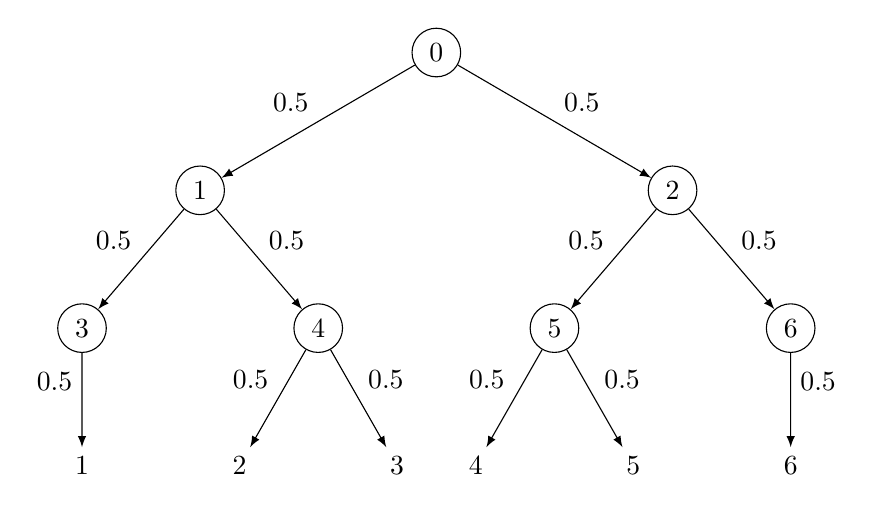
\begin{tikzpicture}[level/.style={sibling distance=60mm/#1, level distance = 1.75cm, -latex}]
\node [circle,draw] (0) {0}
  child {node [circle,draw] (1) {1}
        child {node [circle,draw] (3) {3}
              child {node (d1) {\die1} edge from parent node[above left]{0.5}
              }
        edge from parent node[above left]{0.5}
        }
        child {node [circle,draw] (4) {4}
               child {node (d2) {\die2} edge from parent node[above left]{0.5}
               }
               child {node (d3) {\die3} edge from parent node[above right]{0.5}
               }
        edge from parent node[above right]{0.5}
        }
  edge from parent node[above left]{0.5}
  }
  child {node [circle,draw] (2) {2}
          child {node [circle,draw] (5) {5}
              child {node (d4) {\die4} edge from parent node[above left]{0.5}
              }
              child {node (d5) {\die5} edge from parent node[above right]{0.5}
              }
        edge from parent node[above left]{0.5}
        }
        child {node [circle,draw] (6) {6}
               child {node (d6) {\die6} edge from parent node[above right]{0.5}
        }
        edge from parent node[above right]{0.5}
        }
  edge from parent node[above right]{0.5}
  }
;
\end{tikzpicture}
  \caption{The Dice Example}\label{fig:dice}
\end{figure}

The source code of the dice PRISM model is shown in figure~\ref{fig:dicemodel}. At the beginning, the code indicates that it is describing a discrete-time Markov chain (DTMC). The source code shows a single PRISM module called dice. The variable \textit{s}, which represents the state of the system, can take the values from 0 to 7 and is initialised with the value 0 (line~\ref{dicemodel:s}). The variable \textit{d}, which represents the value of the dice, can range from 0 to 6 and is also initialised with the value 0, meaning that the dice has no value yet (line~\ref{dicemodel:d}).
Each line depicts a state and the probabilities of the transitions, e.g. line~\ref{dicemodel:s1} shows there is a probability of 0.5 of transiting to state 3 or state 4 if we are currently in state 1. The model ends if a value is assigned to the dice, as there are no further transitions from that point on.

\begin{figure}[ht!]
\begin{lstlisting}[language=Prism, ,escapechar=|]
dtmc

module dice

	// local state
	s : [0..7] init 0; |\label{dicemodel:s}|
	// value of the dice
	d : [0..6] init 0;  |\label{dicemodel:d}|
	
	[] s=0 -> 0.5 : (s'=1) + 0.5 : (s'=2);
	[] s=1 -> 0.5 : (s'=3) + 0.5 : (s'=4); |\label{dicemodel:s1}|
	[] s=2 -> 0.5 : (s'=5) + 0.5 : (s'=6);
	[] s=3 -> 0.5 : (s'=1) + 0.5 : (s'=7) & (d'=1);
	[] s=4 -> 0.5 : (s'=7) & (d'=2) + 0.5 : (s'=7) & (d'=3);
	[] s=5 -> 0.5 : (s'=7) & (d'=4) + 0.5 : (s'=7) & (d'=5);
	[] s=6 -> 0.5 : (s'=2) + 0.5 : (s'=7) & (d'=6);
	[] s=7 -> (s'=7);
	
endmodule

\end{lstlisting}
\caption{The Prism Dice Model}
\label{fig:dicemodel}
\end{figure}

\subsubsection{Herman's Self-Stabilisation Algorithm}
The running example we are going to use in this paper (unless explicitly stated otherwise) is a PRISM model of Herman's self-stabilising algorithm, as described in \cite{Kwiatkowska.2012}. The algorithm guarantees that the system recovers from faults in a certain amount of time. Although it is certain that the system self-stabilises eventually, it is very hard to analyse the maximum execution time, which depicts the worst case scenario in this case.
\par Herman's algorithm works with a network of an odd number of identical processes in a ring, ordered anticlockwise. The processes work synchronously and possess a token, which is passed around the ring. The result of a random coin toss decides whether the process keeps the token or passes it on to its neighbour. If a process holds two tokens, they are eliminated. The result is a stable system, where each process has exactly one token and the tokens are passed around forever in the ring. In order to analyse the correctness and the performance of the proposed model, the authors use the tool PRISM Model Checker and invoke probabilistic model checking methods on the model.
\par The proposed methods worked well and proved the correctness of the algorithm. Their findings on the maximum execution time showed, that having 3 tokens, spaced evenly around the ring, always produced the worst-case behaviour. It is stated that probabilistic model checking is extremely useful for checking models of this kind, because simple tools, languages and techniques are provided to model the system. Also, an exhaustive analysis can be done, as opposed to other simulation techniques such as the Monte Carlo simulation. A disadvantage is the restriction of probabilistic model checking to finite state models. Furthermore, the size of the models under analysis are limited to the amount of time and space available.
\par The source code of the model is shown in figure~\ref{fig:hermanmodel}. In this case, seven processes are used in the ring. The step notation in line~\ref{hermanmodel:step} forces all processes to synchronise. The state of each process is depicted by a single two-valued variable (x1-x3). Initially, the value is 1 for all processes. The implementation of this model is straightforward and it is used as a data generator for the input of the AALERGIA implementation.

\begin{figure}[ht!]
\begin{lstlisting}[language=Prism, ,escapechar=|]
dtmc

// module for process 1
module process1

	x1 : [0..1] init 1;
	
	[step] (x1=x3) -> 0.5 : (x1'=0) + 0.5 : (x1'=1); |\label{hermanmodel:step}|
	[step] !(x1=x3) -> (x1'=x3);
	
endmodule

// add further processes through renaming
module process2 = process1[x1=x2, x3=x1 ] endmodule
module process3 = process1[x1=x3, x3=x2 ] endmodule


\end{lstlisting}
\caption{The Prism Herman 3 Model}
\label{fig:hermanmodel}
\end{figure}

\subsection{AALERGIA}
ALERGIA\cite{Carrasco.1994} was introduced by Rafael C. Carrasco and Jose Oncina in 1994. They proposed an algorithm which is capable of identifying any stochastic deterministic regular language by using a prefix tree acceptor and merging the states in O(|S|\textsuperscript{3}), where |S| is the size of the sample. This is especially useful for learning automaton in realistic situations. They based their approach on previous work from Oncina\cite{Oncina92}. ALERGIA has been extended in many ways, one of many is called AALERGIA\cite{Mao.}.
\par The reason for creating AALERGIA was to show that the methods for learning probabilistic automata can be adapted for learning Markov Chain system models for verification. The algorithm also leads to stronger consistency for learning in the limit than previous implementations and the authors analyse how the convergence of the learned model relates to the convergence of probability estimates for system properties. This enables us to use the learned model for probabilistic linear temporal logic (PLTL) model checking.
\par However, there is still room for improvement, as shown in a competition called PAutomaC\footnote{hai.cs.umbc.edu/icgi2012/challenge/Pautomac/index.php} by the winner team\cite{Shibata_the11th}. They introduced a new criterion for merging states based on marginal probability by greedily merging states if it increases the probability of the automaton.
\par In this paper, we take AALERGIA and the provided MATLAB implementation\footnote{http://mi.cs.aau.dk/code/aalergia}, implement it in python and experiment with it. In order to get a better idea of the way the implementation works, we will describe it in detail and a running example for better replicability is used throughout this section. The implementation of the algorithm consists of several parts, which are depicted in the figure~\ref{fig:diaAalergia}.

\begin{figure}[H]
\begin{center}
    \smartdiagramset{
        back arrow disabled=true,
        module minimum width=2cm,
    module minimum height=2cm,
    module x sep=3cm,
    text width=2cm,
    }
   \smartdiagram[flow diagram:horizontal]{Training Data, Prefix Tree Acceptor, Golden Section Search, AALERGIA, DLMC}
\end{center}
    \captionof{figure}{The Flow Diagram AALERGIA}
     \label{fig:diaAalergia}
\end{figure}

\subsubsection{Training Data}
The data used to learn the Deterministic Labeled Markov Chain (DLMC) is supplied in the form of a comma separated values file, which contains the training set and the alphabet to be used. The alphabet consists of a finite 1$\times$N-cell array, where each column contains one letter in the alphabet. The training set consist of a finite N$\times$1-cell array, where each row contains sequences of symbols generated from the model, separated by commas.
\paragraph{Dataset Generator} It is easy to generate datasets by using the command line version of PRISM. It is possible to generate random paths through a model by specifying the model file, an output file and the path to be generated (for instance, how many steps should be processed). The output file can then be used as input file for the AALERGIA implementation.
\par The running example we are going to use is a self-stabilizing ring network with 3 processes.
Table~\ref{table:trainingsSet} shows the beginning of the training set, generated by the PRISM modelchecker, which contains 50 Sequences in total.  In our case, each symbol in the training set represents the states in the ring at a given moment. For example, the symbol 001 shows that process 3 is in the state 1 and process 1 and 2 are in the state 0.

\begin{table}[ht!]
\centering
\begin{tabular}{|l|l|}
\hline
\gray & \gray  1                                 \\ \hline
\gray 1& 000,001,                                    \\ \hline
\gray 2& 000,011,100,010,101,010,001,100,010,101,   \\ \hline
\gray 3& 000,101,                                    \\ \hline
\gray 4& 000,111,010,001,110,011,101,010,001,110,011, \\ \hline
\gray 5& 000,111,011,101,110,001,                    \\ \hline
\gray 6& 000,101,010,101,110,011,100,011,101,110,    \\ \hline
\end{tabular}
\caption{The Training set}
\label{table:trainingsSet}
\end{table}

Table~\ref{table:alphabet} shows the alphabet, which consists of 8 symbols from 000 to 111.

\begin{table}[ht!]
\centering
\begin{tabular}{|l|l|l|l|l|l|l|l|l|}
\hline
\gray & \gray 1 & \gray 2 & \gray 3 & \gray 4 & \gray 5 & \gray 6 & \gray 7 & \gray 8 \\ \hline
\gray 1 & 000 & 001 & 010 & 011 & 100 & 101 & 110 & 111 \\ \hline
\end{tabular}
\caption{The Alphabet}
\label{table:alphabet}
\end{table}

\subsubsection{Frequency Prefix Tree Acceptor}
After loading the training set and the alphabet into the workspace, the Frequency Prefix Tree Acceptor (FPTA) is created. A deterministic frequency finite automaton (DFFA) is a tuple $A = \langle \Sigma, Q, I\textsubscript{fr}, F\textsubscript{fr}, \delta\textsubscript{fr}, \delta \rangle$ where $ \Sigma $ = the finite alphabet, $Q$ = the finite set of states, $I\textsubscript{fr}$ = the initial state frequencies, $F\textsubscript{fr}$ = the final state frequencies, $\delta\textsubscript{fr}$ = the frequency transition function and $ \delta$ = the transition function.

Figure~\ref{fig:fptadice} shows how a simplified FPTA for the in section~\ref{section:diceprograms} described dice model looks like. The sample S is a multiset of size 20. S = \{(SH,1), (SHHH,1), (SHHHD\textsubscript{1},1), (SHHD\textsubscript{1},2), (SHHD\textsubscript{1}D\textsubscript{1},1), (SHT,2), (SHTD\textsubscript{2},1), (SHTD\textsubscript{2}D\textsubscript{2},1), (SHTD\textsubscript{3},1), (ST,1), (STH,2), (STHD\textsubscript{4},1), (STHD\textsubscript{5},1), (STT,2), (STTD\textsubscript{6},2)\}. The letter H stands for heads, the letter T stands for tails and D1 - D6 stands for the different dice values. The numbers in the state indicates the number of the occurrence of the event, whereas the number on the transitions illustrates the count of all events below it.

\begin{figure}[ht!]
  \centering
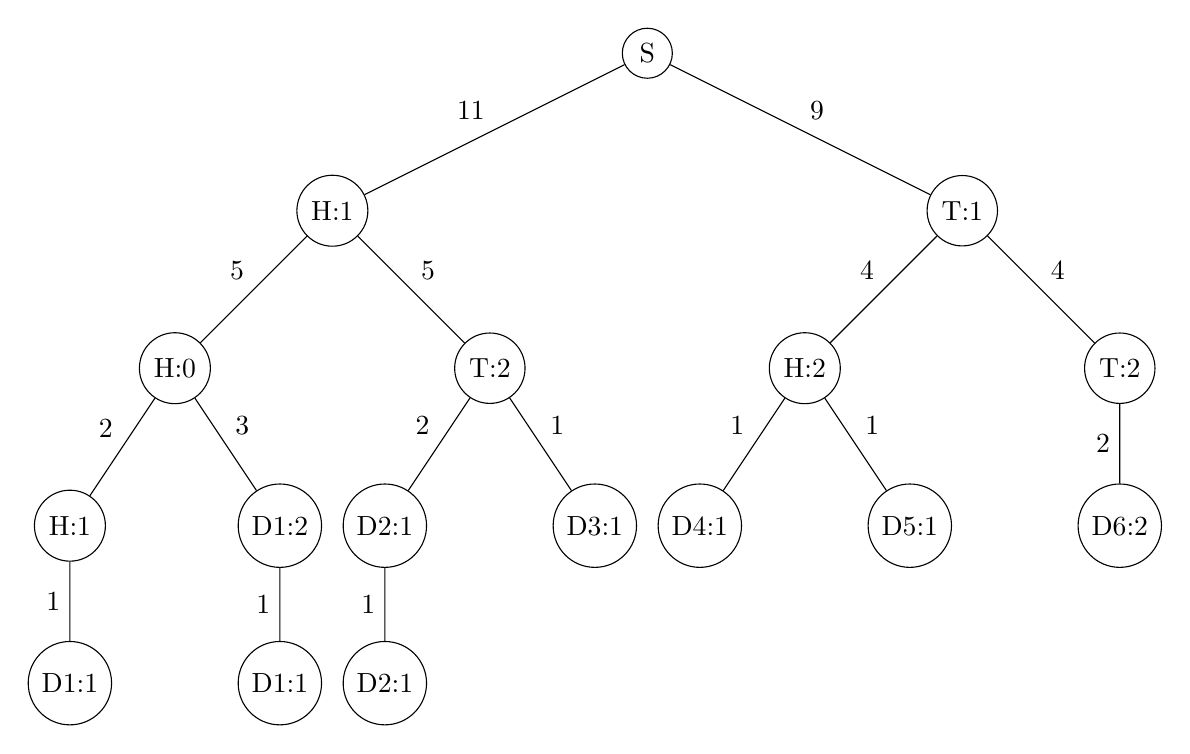
\begin{tikzpicture}[level/.style={sibling distance=80mm/#1, level distance = 2cm}]
\node [circle,draw] (s){S}
  child {node [circle,draw] (h) {H:1}
        child {node [circle,draw] (hh) {H:0}
        child {node [circle,draw] (hhh) {H:1}
              child {node [circle,draw] (hhhd1) {D1:1} edge from parent node[left]{1}}
        edge from parent node[above left]{2}
        }
        child {node [circle,draw] (hhd1) {D1:2}
              child {node [circle,draw] (hhd1d1) {D1:1} edge from parent node[left]{1}}
        edge from parent node[above right]{3}
        }
        edge from parent node[above left]{5}
        }
        child {node [circle,draw] (ht) {T:2}
              child {node [circle,draw] (htd2) {D2:1}
                    child {node [circle,draw] (htd2d2) {D2:1} edge from parent node[left]{1}}
              edge from parent node[above left]{2}
              }
              child {node [circle,draw] (htd3) {D3:1} edge from parent node[above right]{1}}
              edge from parent node[above right]{5}
        }
  edge from parent node[above left]{11}
  }
  child {node [circle,draw] (t) {T:1}
         child {node [circle,draw] (th) {H:2}
               child {node [circle,draw] (ttd4) {D4:1} edge from parent node[above left]{1}}
               child {node [circle,draw] (ttd5) {D5:1} edge from parent node[above right]{1}}
         edge from parent node[above left]{4}
         }
         child {node [circle,draw] (tt) {T:2}
               child {node [circle,draw] (ttd6) {D6:2} edge from parent node[left]{2}}
         edge from parent node[above right]{4}
         }
  edge from parent node[above right]{9}
  }
;
\end{tikzpicture}
  \caption{The FPTA for the DICE model}\label{fig:fptadice}
\end{figure}

\par Algorithm~\ref{alg:fpta} shows how the creation of the FPTA is implemented in the AALERGIA package. The code starts by sorting the training set and by removing double occurrences (line~\ref{fpta:sort}).
After that, a for-loop iterates through the sorted strings and splits them at each comma (line~\ref{fpta:BeginForPrefix} -~\ref{fpta:EndForPrefix}).
This creates all the prefixes from the training set and adds them to the cell array named \emph{prefix}, as shown in Table~\ref{table:prefix}.
\begin{table}[ht!]
\centering
\begin{tabular}{|l|l|}
\hline
\gray & \gray  1                                 \\ \hline
\gray 1&000,000,010,001,100,011,101,110,001,110,001,110,011,101,010,001,100,011,100,010,001,   \\ \hline
\gray 2&000,000,010,001,100,011,101,110,001,110,001,110,011,101,010,001,100,011,100,010,   \\ \hline
\gray 3&000,000,010,001,100,011,101,110,001,110,001,110,011,101,010,001,100,011,100,   \\ \hline
\gray 4&000,000,010,001,100,011,101,110,001,110,001,110,011,101,010,001,100,011,   \\ \hline
\gray 5&000,000,010,001,100,011,101,110,001,110,001,110,011,101,010,001,100,   \\ \hline
\gray 6&000,000,010,001,100,011,101,110,001,110,001,110,011,101,010,001,   \\ \hline
\gray 7&000,000,010,001,100,011,101,110,001,110,001,110,011,101,010,   \\ \hline
\gray 8&000,000,010,001,100,011,101,110,001,110,001,110,011,101,   \\ \hline
\gray 9&000,000,010,001,100,011,101,110,001,110,001,110,011,   \\ \hline
\gray 10&000,000,010,001,100,011,101,110,001,110,001,110,   \\ \hline
\gray 11&000,000,010,001,100,011,101,110,001,110,001,   \\ \hline
\end{tabular}
\caption{The Prefixes}
\label{table:prefix}
\end{table}

\begin{algorithm}[]
\caption{Create the FPTA}\label{alg:fpta}
\begin{algorithmic}[1]
\item \textbf{Input:} the $\sum$ and a set of strings S (training data)
\item \textbf{Output:} a DFFA A and a sorted set of strings U

\State $\textit{U} \gets \text{sort}(\textit{S})$ \label{fpta:sort}
\State $\textit{prefixes} \gets \textit{U}$
\State $\textit{F\textsubscript{fr}} \gets \text{string\_count}(\textit{U})$
\For{$\texttt{u} \in \texttt{U}$} \label{fpta:BeginForPrefix}
        \State $\textit{index} \gets \text{find positions of ``,'' in }\textit{u}$

        \While{$index > 0$}
          \State $\textit{substr} \gets \textit{substring(1:index)}$
         \If {$\textit{substr} \not\in \textit{prefix}$}
   	 \State $\textit{prefixes(end+1)} \gets \textit{substr}$
        \EndIf
           \State $\textit{index} \gets \textit{index-1}$
       \EndWhile
\EndFor \label{fpta:EndForPrefix}

\State $\textit{prefixes} \gets \text{width\_first\_sort}(\textit{prefixes})$ \label{fpta:widthSort}
\State $\textit{predecessor} \gets \text{find\_predecessor}(\textit{prefixes})$ \label{fpta:findPredecessor}

\For{$\texttt{p} \in \texttt{prefixes}$} \label{fpta:BeginForFreq}
\State $\textit{sym} \gets \textit{get\_symbol(p)}$
\State $\textit{pre} \gets \textit{predecessor(p)}$

\State $\textit{freq\_trans\_matrix\textsuperscript{1} (pre, sym)} \gets \textit{predecessor(p)}$
\State $\textit{frequency\_transition} \gets \textit{freq\_trans\_matrix\textsuperscript{2} (pre, sym)} $
\State $\textit{frequency\_transition} \gets \textit{frequency\_transition} + \textit{frequency(p)}$

 \While{$pre$}
          \State update\_freq\_trans\_matrix(\textit{p, pre})
          \State $\textit{pre} \gets \textit{predecessor(p)}$
   \EndWhile

\EndFor \label{fpta:EndForFreq}

\State $\textit{init\_states} \gets  \textit{freq\_trans\_matrix\textsuperscript{1}(1, all)}$
\State \Return \textit{A}  \label{fpta:return}
\end{algorithmic}
\end{algorithm}

In our example, the dimension of  \emph{prefix} is 494x1 and contains all unique prefixes of the training set for further evaluation.
The cell array \emph{prefix} is sorted by width-first-sort (line~\ref{fpta:widthSort}). The shortest strings are at the beginning of the array and the largest at the end of the array, as shown in Table~\ref{table:sortPrefix}.

\begin{table}[ht!]
\centering
\begin{tabular}{|l|l|}
\hline
\gray & \gray  1                                 \\ \hline
\gray 1&000,         \\ \hline
\gray 2&000,000,     \\ \hline
\gray 3&000,001,     \\ \hline
\gray 4&000,010,     \\ \hline
\gray 5&000,011,     \\ \hline
\gray 6&000,100,     \\ \hline
\gray 7&000,101,     \\ \hline
\gray 8&000,110,     \\ \hline
\gray 9&000,111,     \\ \hline
\gray 10&000,000,010, \\ \hline
\gray 11&000,000,100, \\ \hline
\gray 12&000,000,111, \\ \hline
\gray 13&000,001,100, \\ \hline
\gray 14&000,001,110, \\ \hline
\end{tabular}
\caption{The Sorted Prefix Array}
\label{table:sortPrefix}
\end{table}

The function \emph{find\_predecessor} searches through the \emph{prefixes} array and saves all the predecessors in the corresponding array (line~\ref{fpta:widthSort}). In the end, a for-loop over all the prefixes is executed in order to find all transitions and their frequencies respectively. The values are saved into the \emph{freq\_trans\_matrix}  (line~\ref{fpta:BeginForFreq} -~\ref{fpta:EndForFreq}). This Matrix contains 2 elements: the first element is the transition matrix, which contains all the transition between the states. The second element is a matrix, which contains all the frequencies between the states.

The returned object DFFA (line~\ref{fpta:return}) has the following members:
\begin{itemize}
      \item a finite set of states
      \item the labels of the states
      \item the alphabet
      \item the initial state
      \item the initial state frequency
      \item the final state frequency
      \item the frequency transition matrix
      \item RED (later used for merging) \me{be more comprehensive about RED set}
      \item BLUE (later used for merging) \me{likewise}
   \end{itemize}

Table~\ref{table:transitionMatrix} shows how the first element of the frequency transition matrix (the transition matrix) is structured. The columns represent the 8 symbols, the rows the different states. For example,  row number 2, column 1 shows the number 3. This indicates that state 2 and symbol 1 lead to state 3. The second element of the frequency transition matrix has the same dimensions as the first element and follows the same logic, but instead of transitions it contains the frequencies.

\begin{table}[ht!]
\centering
\begin{tabular}{|l|l|l|l|l|l|l|l|l|}
\hline
\gray &\gray 1 & \gray 2  & \gray 3  & \gray 4 & \gray 5  & \gray 6  & \gray 7  & \gray 8  \\ \hline
\gray 1&2 & 0  & 0  & 0 & 0  & 0  & 0  & 0  \\ \hline
\gray 2&3 & 4  & 5  & 6 & 7  & 8  & 9  & 10 \\ \hline
\gray 3&0 & 0  & 11 & 0 & 12 & 0  & 0  & 13 \\ \hline
\gray 4&0 & 0  & 0  & 0 & 14 & 0  & 15 & 0  \\ \hline
\gray 5&0 & 16 & 0  & 0 & 0  & 17 & 0  & 0  \\ \hline
\end{tabular}
\caption{The Transition Matrix}
\label{table:transitionMatrix}
\end{table}

\subsubsection{Normalization}

The algorithm~\ref{alg:normalize} shows how a DFFA is converted into a deterministic probabilistic finite automaton (DPFA). The computation is pretty straightforward. As input, the algorithm takes a well defined DFFA, that means that the number of strings entering and leaving a given state is identical. The probabilistic transition matrix (line~\ref{normalize:ptm}) is identical to the frequency transition matrix, but its second element contains the probabilities of the transitions instead of the frequencies of the transitions.

The algorithm searches through the frequency transition matrix, sums up the frequencies of the transitions and adds them to the frequency of the state itself in order to get the total number of frequencies (line~\ref{normalize:sum}). Following that, the frequency of each transition and of the state is divided by the total number of total frequencies, which results in the corresponding probabilities for the transitions. (line~\ref{normalize:divide}).

\begin{algorithm}[H]
\caption{Create a DPFA from a DFFA}\label{alg:normalize}
\begin{algorithmic}[1]
\item \textbf{Input:} a well defined DFFA
\item \textbf{Output:} corresponding DPFA

\For{$q \in Q$}
        \State $\textit{freq\_state} \gets \textit{dffa.finalStateFrequency(q)}$
        \State $\textit{ptm\textsuperscript{1}} \gets \textit{dffa.frequencyTransitionMatrix\textsuperscript{1}}$ \label{normalize:ptm}
         \State $\textit{freq\_trans} \gets \textit{dffa.frequencyTransitionMatrix\textsuperscript{2}(q, all)}$
         \State $\textit{freq\_total} \gets \textit{freq\_trans + freq\_state}$  \label{normalize:sum}

         \If {$\textit{freq\_total} > 0$}
   	 \State $\textit{ptm\textsuperscript{2}(node, index)} \gets \frac{freq\_trans}{freq\_total}$ \label{normalize:divide}
   	  \State $\textit{fsp(q)} \gets \frac{freq\_state}{freq\_total}$
       \EndIf
\EndFor
\State \Return \textit{DPFA(dffa, fsp, ptm)}
\end{algorithmic}
\end{algorithm}

\subsubsection{Golden Section Search}

First, we need to search for a left and right border of $\varepsilon$ in order to get a region for our golden section search. This is done by the following algorithm~\ref{alg:findregion}. In order to save space, the algorithm only explains how to find the left border of the region. The right border is found the same way, with some minor modifications. The algorithm iteratively calculates BIC-scores for the values of $\varepsilon$. For each run of the while-loop, the $\varepsilon$ is multiplied by 0.5 until a left border is found. If the new $\varepsilon$ produces a Bayesian Information Criterion(BIC)-score larger than the previous $\varepsilon$ (line~\ref{findregion:scorelarger}), it essentially means that we found a right border, but the left border is further to the left and we need to search again. If the new score is the same as the old score  (line~\ref{findregion:scorethesame}), we search again. If the value of the score doesn't change for 5 consecutive tries, we break the loop and take the last value of $\varepsilon$ as our left border. Last but not least, if the new score is smaller than the old score (line~\ref{findregion:scoresmaller}), we found the left border and can continue searching for the right border (not shown in the pseudo code).
\paragraph{BIC Score} This is a measure that can be used to evaluate the learned model. It creates a score that is calculated on the likelihood minus a penalty term for the model complexity. The BIC score of a given DLMC A given data $S[n]$ is defined in formula~\ref{eq:bic}

  \begin{equation} \label{eq:bic}
  BIC(A | S[n]) := log(P_A(S[n])) - 1/2 | A | log(N)
  \end{equation}

In this formula, $|A|$ depicts the size of A and $N = \sum l_i$ is the total size of the data.

\begin{algorithm}[H]
\caption{Find $\varepsilon$-region}\label{alg:findregion}
\begin{algorithmic}[1]
\item \textbf{Input:} the DFFA
\item \textbf{Output:} the region for $\varepsilon$, scores, epsilon\_values

\State $\varepsilon \gets \textit{1}$
\State \textit{score} $\gets$ calculate\_BIC\_Score($\varepsilon$, \textit{dffa})
\State $new\_\varepsilon \gets \varepsilon * 0.5$

 \While{$new\_\varepsilon > 0$}

       \State \textit{new\_score} $\gets$ calculate\_BIC\_score(new\_$\varepsilon$, \textit{dffa})

         \If {\textit{new\_score > score}}  \label{findregion:scorelarger}
         \State $\textit{region\_right} \gets \varepsilon$
         \State $\varepsilon \gets new\_\varepsilon$
         \State $ new\_\varepsilon \gets new\_\varepsilon * 0.5$
         \State $\textit{score} \gets \textit{new\_score} $

         \ElsIf {\textit{new\_score = score}} \Comment{do this max. 5 times} \label{findregion:scorethesame}
   	 \State $\varepsilon \gets new\_\varepsilon$
         \State $ new\_\varepsilon \gets new\_\varepsilon * 0.5$
         \State $\textit{score} \gets \textit{new\_score} $

      \Else \label{findregion:scoresmaller}
      \State $\textit{region\_left} \gets new\_\varepsilon$
        \State break
       \EndIf

  \EndWhile

  \State ...
  \State ...

\State \Return \textit{region\_right, region\_left}
\end{algorithmic}
\end{algorithm}

Table~\ref{table:region} shows the values of the left and right border of $\varepsilon$. The algorithm ran only once for the left border ($\varepsilon$ startes with 1 and is halfed every run) and 5 times for the right border, since the scores always stayed the same. Table~\ref{table:bicscores} shows the BIC scores and table~\ref{table:epsilonvalues} shows the corresponding $\varepsilon$ values. For example, we calculated the BIC score for $\varepsilon = 0.5$ and the result was $-1.5769e+03$.

\begin{table}[ht!]
\centering
\begin{tabular}{|l|l|l|}
\hline
\gray &\gray 1 & \gray 2 \\ \hline
\gray 1&0.5 & 64 \\ \hline
\end{tabular}
\caption{The Search Region}
\label{table:region}
\end{table}

\begin{table}[ht!]
\centering
\begin{tabular}{|l|l|l|l|l|l|l|l|l|}
\hline
\gray &\gray 1 & \gray 2 & \gray 3 & \gray 4 & \gray 5 & \gray 6 & \gray 7 & \gray 8 \\ \hline
\gray 1&-840.608 & -1.5769e+03 & -840.608 & -840.608 & -840.608 & -840.608 & -840.608 & -840.608 \\ \hline
\end{tabular}
\caption{The BIC scores}
\label{table:bicscores}
\end{table}

\begin{table}[ht!]
\centering
\begin{tabular}{|l|l|l|l|l|l|l|l|l|}
\hline
\gray &\gray 1 & \gray 2 & \gray 3 & \gray 4 & \gray 5 & \gray 6 & \gray 7 & \gray 8 \\ \hline
\gray 1&1 & 0.5 & 2 & 4 & 8 & 16 & 32 & 64 \\ \hline
\end{tabular}
\caption{The Epsilon values}
\label{table:epsilonvalues}
\end{table}

After having found the region, the golden section search can begin. Algorithm~\ref{alg:goldensection} shows how it is implemented. Basically, the algorithm uses the golden ratio on our 2 borders a1 and a2 and tries to find a maximum (the highest BIC score) between these 2 values. If it exists, the section that contains the maximum is selected as new region and the search is started again, until the recursion reaches depth 3 or the condition at line~\ref{golden:condition} is fulfilled. At line~\ref{golden:calcratio},~\ref{golden:calcratio2} we calculate the 2 values a1,a2 for our golden ratio, given the region r1,r2. After that, the corresponding BIC scores f1,f2 are calculated(line~\ref{golden:bicscore},~\ref{golden:bicscore2}). If the distance between the 2 values a1,a2 is small enough, we stop the recursion and the average score between the 2 values is taken as a good $\varepsilon$ (line~\ref{golden:average}). If f1 is smaller than f2, the maximum has to be between a1 and r2 and a new golden section search is started. If it is the other way around and f1 is larger than f2, the maximum is between r1 and a2 and we start the search with these values.
If it happens that the score of f1 and f2 is exactly the same, we need to make sure, that the recursion is not endless (line ~\ref{golden:limit}). We check if f1 is larger than the largest score we already calculated. Should this be the case, the maximum is between a1 and a2 (line~\ref{golden:maxscores}). Lastly, if we do not have any luck and we have not found a maximum so far, we simply start 2 new golden searches for the left (r1, a1) and the right (a2, r2) region respectively (line~\ref{golden:leftregion},~\ref{golden:rightregion}). In the end, the algorithm returns a suggestion for a good $\varepsilon$ as shown in Table~\ref{table:goodepsilon}, which we use as input parameter ($\alpha$) for our merging algorithm.

\begin{table}[ht!]
\centering
\begin{tabular}{|l|l|}
\hline
\gray &\gray 1 \\ \hline
\gray 1&64 \\ \hline
\end{tabular}
\caption{The Epsilon}
\label{table:goodepsilon}
\end{table}

\begin{algorithm}[H]
\caption{Golden\_section\_search}\label{alg:goldensection}
\begin{algorithmic}[1]
\item \textbf{Input:} region, dffa, scores
\item \textbf{Output:} good\_eps, scores, epsilon

\State $\textit{good\_eps} \gets \textit{0}$
\State $\textit{r1} \gets \textit{region(1,1)}$
\State $\textit{r2} \gets \textit{region(1,2)}$

 \While{\textit{true}}

       \State $\textit{a1} \gets \textit{r1 + 0.382(r2-r1)}$ \label{golden:calcratio}
       \State $\textit{a2} \gets \textit{r2 + 0.618(r2-r1)}$ \label{golden:calcratio2}
       \State \textit{f1} $\gets$ calculate\_BIC\_score(\textit{a1,dffa}) \label{golden:bicscore}
       \State \textit{f2} $\gets$ calculate\_BIC\_score(\textit{a2, dffa}) \label{golden:bicscore2}

         \If {\textit{|a1-a2| < 0,00001}} \label{golden:condition}
       \State $\textit{good\_eps} \gets \textit{(a1 + a2) / 2}$   \label{golden:average}
        \State \Return
       \EndIf

        \If {\textit{f1 < f2}}
        \State $\textit{region} \gets \textit{region(a1, r2)}$
        \State \textit{good\_eps, scores, epsilon} $\gets$ Golden\_section\_search(\textit{region, dffa, scores})
       \State \Return

        \ElsIf {\textit{f1 > f2}}
        \State $\textit{region} \gets \textit{region(r1, a2)}$
        \State \textit{good\_eps, scores, epsilon} $\gets$ Golden\_section\_search(\textit{region, dffa, scores)}
        \State \Return

      \Else
        \If {\textit{recursion\_depth = 3}}  \label{golden:limit}
        \State \Return
        \EndIf

        \If {\textit{f1 > max(scores)}}  \label{golden:maxscores}
        \State $\textit{new\_region} \gets \textit{a1, a2)}$
        \State \textit{good\_eps, scores, epsilon} $\gets$ Golden\_section\_search(\textit{new\_region, dffa, scores)}
        \State \Return

        \Else
          \State $\textit{regionL} \gets \textit{region(r1, a1)}$
          \State $\textit{regionR} \gets \textit{region(a2, r2)}$
        \State \textit{good\_eps, scores, epsilon} $\gets$ Golden\_section\_search(\textit{regionL, dffa, scores)} \label{golden:leftregion}
         \State \textit{good\_eps, scores, epsilon} $\gets$ Golden\_section\_search(\textit{regionR, dffa, scores)} \label{golden:rightregion}
        \State \Return
        \EndIf
       \EndIf

  \EndWhile
\end{algorithmic}
\end{algorithm}

\subsubsection{Merging }

After having calculated a good $\alpha$ value, we can finally start the AALERGIA algorithm. RED is a set of states, that is already revised, whereas BLUE is the set of states that we need to look at. The RED set starts with the initial state (line~\ref{aalergia:redstart}) and BLUE gets all its successors (line~\ref{aalergia:bluestart}). After that, we loop through all the elements of BLUE and check if we can merge it with the AALERGIA\_compatible criterion (line~\ref{aalergia:criterion}). If the states are compatible, we can merge them and the tree becomes smaller, if not, we promote the state to the RED set (line~\ref{aalergia:promote}) and exclude it from the BLUE set (line~\ref{aalergia:excludeblue}). In the end, we get a merged DFFA with a good BIC score. Further details on the AALERGIA\_compatible criterion can be found at \cite{Mao.}

\begin{algorithm}[H]
\caption{AALERGIA}\label{alg:aalergia}
\begin{algorithmic}[1]
\item \textbf{Input:}  a DFFA, a DPFA, the alpha
\item \textbf{Output:} the merged DFFA

\State $\textit{RED} \gets \textit{dffa.initial\_state}$ \label{aalergia:redstart}
\State $\textit{BLUE} \gets \textit{freq\_trans\_matrix\textsuperscript{1}(dffa.initial\_state, all)}$ \label{aalergia:bluestart}
\State \textit{promote} $\gets$ \textit{1}

 \While{BLUE is not empty}

 \State $\textit{BLUE} \gets$ sort(\textit{BLUE})
 \State $\textit{q\_b} \gets \textit{BLUE(1)}$
 \State $\textit{BLUE}$.remove\textit{(q\_b)}
 \State $\textit{same\_label\_ind} \gets $find\_same\_labels(\textit{RED, q\_b)}

 \For{$ind \in same\_label\_ind$}
        \State $\textit{q\_r} \gets \textit{RED(ind)}$
        \State $\textit{threshold} \gets$ calculate\_compatible\_params(\textit{dffa, q\_r, q\_b, alpha})

        \If {AALERGIA\_compatible(\textit{dffa, dpfa, q\_r, q\_b, alpha, threshold})} \label{aalergia:criterion}
          \State \textit{dffa\_merged} $\gets$ AALERGIA\_merge(\textit{RED, BLUE, q\_r, q\_b})
          \State \textit{promote} $\gets$ \textit{0}
          \State break
        \EndIf
\EndFor

     \If  {promote}
          \State \textit{RED} $\gets$ \textit{q\_b} and \textit{RED} \label{aalergia:promote}
        \EndIf

    \State \textit{successors} $\gets$ \textit{dffa\_merged.freq\_trans\_matrix\textsuperscript{1}}(\textit{RED, all})
    \State \textit{BLUE} $\gets$ all \textit{successors} not in \textit{RED} \label{aalergia:excludeblue}
  \EndWhile
\end{algorithmic}
\end{algorithm}

\subsubsection{Perplexity}
%%% Section RELATED WORK
\newpage
\section{Related Work}
\me{The contest you were looking at. write three paragraphs each of which dedicated to one of the top three approaches; cite the publications (Worst to best).}
\me{The continue the discussion on SHIBATA and why it is winning every major contest in this field  PAutomataC 2012, CONTEST 2016.}

\section{Meat}
\me {a case study on wireless sensory networks.}



\newpage
\section{Evaluation}
\me {compare the findings about the case study with real-world scenario and the knowledge of an expert in the field of wireless sensory networks.}



\newpage
\section{Conclusions}
\me{the approach is good; but!}

\appendix
 \bibliographystyle{ieeetr}
 \bibliography{sources}

\end{document} 